\chapter{Introducción}
\label{champ:intro}
\bigskip
\barra
\bigskip

Por años se han utilizado las computadoras como herramientas para la solución, aproximación o simulación de problemas científicos reales, los cuales tienen una o varias de las siguientes características: son complejos, requieren de un gran número de cálculos o manipulan grandes volúmenes de datos. Lo anterior fue la razón por la cual nació la computación científica la cual es una actividad multidisciplinaria en la cual se hace uso de métodos y técnicas computacionales para dar soluciones exactas o aproximadas con la premisa de que al utilizar las computadoras el tiempo para obtener resultados es menor.\\

La simulación por computadora es una herramienta altamente utilizada debido a que nos permite obtener soluciones aproximadas sobre escenarios de la vida real, varios ramas de la ciencia se auxilian de simulaciones por computadora para lograr mejores resultados en experimentos reales basándose en la información obtenida de simulaciones. Cuando se habla de simulación por computadora, est\'a inherente que se requiere de un modelo el cual nos ayude a abstraer características y limitaciones de un problema real. Adicionalmente de que la simulación por computadora nos puede permitir generar experimentos con mayor exactitud, \'esta también nos puede ayudar a disminuir riesgos y ahorrar recursos.\\

En particular este proyecto hace énfasis en la simulación de materiales porosos, donde tal y como su nombre lo dice son materiales que tienen poros o huecos, estos poros son de distintos tamaños y se encuentran distribuidos en todo el material con la peculiaridad de que dichos poros se encuentran conectados entre s\'i. Debido a las características que tienen los materiales porosos son altamente utilizados en la industria, al estudiar la estructura y propiedades de estos materiales y adicionalmente con la simulación por computadora se pueden encontrar nuevas aplicaciones y usos industriales.\\

Varios m\'etodos para la simulaci\'on de redes porosas han sido propuestos; sin embargo, muy pocos validan el cumplimiento de las restricciones geom\'etricas que surgen al conectar dos o mas poros adyacentes, en donde no debe existir interferencia espacial entre ellos. El validar este tipo de restricciones nos ayuda a crear redes porosas m\'as realistas,
pero el procesamiento de millones o billones de datos que pueden representar los poros de una red, junto con la complejidad algor\'itmica para hacer respetar las restricciones geom\'etricas, se vuelve un reto computacional importante.\\

Por lo general la computación científica hace uso  del computo de alto rendimiento(computo paralelo) a través de modelos de programación paralela, los cuales permiten  el uso eficiente de los recursos computacionales para disminuir el tiempo en la obtenci\'on de resultados.
El c\'omputo paralelo fue impulsado gracias a los avances tecnológicos como lo fueron las computadoras multi-procesador o los primeros clusters(Beowulf), en ambas arquitecturas hubo un avance significativo; en la primera fue la incorporación de más de un procesador en una misma tarjeta y en la segunda fue el uso de la capacidad de computo de computadoras independientes a través de su interconexión(cluster). En la actualidad el computo paralelo va cobrando mayor fuerza y adem\'as conforme pasa tiempo se est\'a volviendo más accesible y por lo mismo se est\'a aplicando en un mayor número de áreas de conocimiento. En particular, para aplicar el computo paralelo en un problema, se requiere elegir una arquitectura y un técnica de programación. Las arquitecturas más utilizadas para el cómputo paralelo o de alto rendimiento son: multi-procesador, multi-núcleo, gpus, clusters y grids. Respecto a técnicas de programación,  las podemos dividir en 3 grandes grupos: la programación con memoria compartida, la programación con memoria distribuida o programación híbrida.\\


Cuando se utilizan arquitecturas multi-núcleo, la mejor opci\'on de programación paralela se realiza a través de la creaci\'on de hilos(tareas computacionales), para que las unidades de procesamiento puedan accesar a la memoria de manera compartida. Dos de las tecnologías más utilizadas para el manejo de hilos son: Posix Threads\cite{ref13} y OpenMP\cite{ref6}, ambos siguen el modelo fork-join, sin embargo OpenMP proporciona una interfaz de alto nivel que permite al programador concentrar la mayor parte de su esfuerzo en resolver el problema de aplicaci\'on y no en aspectos técnicos de creaci\'on expl\'icita de hilos y manejo de mecanismos de sincronizaci\'on, que en ocasiones generan errores que no se relacionan con el problema que se quiere resolver. Ademas OpenMP es un estándar avalado por diversas empresas internacionales y se encuentra soportado por los principales compiladores de C/C++ y Fortran.\\ 

Este trabajo contribuye a la simulaci\'on paralela de redes porosas que consideran el cumplimiento de restricciones geom\'etricas entre poros adyacentes, usando una arquitectura multi-núcleo y OpenMP. Se proponen dos algoritmos paralelos que permiten construir redes porosas haciendo que varios hilos de ejecuci\'on trabajen en diferentes regiones de una red porosa c\'ubica para disminuir el tiempo de simulaci\'on. El alcance de este proyecto se enfoca en la comparaci\'on de esas dos propuestas. \\

%\section{Organización de la Idónea Comunicación de Resultados}
%En el Capítulo \ref{champ:intro} se da una introducción sobre los materiales porosos y algunas de sus aplicaciones, también se habla ligeramente sobre el Principio de Construcción y las Restricciones Geométricas y algunas de las ventajas de estas últimas, adicionalmente se habla u poco sobre el computo paralelo y su aplicación en la simulación por computadora, al final se agrega el objetivo general y los objetivos específicos de este proyecto; 

En el Cap\'itulo siguiente se presentan los conceptos b\'asicos relacionados con la simulaci\'on de las redes porosas. Posteriormente, el Cap\'itulo \ref{champ:objetivos} presenta los objetivos de este trabajo. En el Capítulo \ref{champ:relatedwork} se muestra en forma de resumen el trabajo relacionado en cuanto a algoritmos para la construcción de redes porosas que se basan en MDSE y las ventajas del c\'omputo paralelo sobre sistemas de memoria compartida utilizando arquitecturas multi-core. En el Capítulo \ref{champ:BSGR} se presentan dos algoritmos secuenciales para la creación de redes porosas sujetas a las restricciones geométricas. En el Capítulo \ref{champ:PBSGR} se presenta la paralelización de los dos algoritmos secuenciales para la creación de redes porosas sujetas las restricciones geométricas. En el Capítulo \ref{champ:results} se presentan la plataforma de pruebas y los resultados obtenidos así como una análisis de los mismos; por último, en el Capítulo \ref{champ:conclusions} se presentan las conclusiones y el trabajo futuro.


\chapter{Simulaci\'on de Redes Porosas}
\label{champ:construction}
\bigskip
\barra
\bigskip


\section{Modelado de Redes Porosas}
\label{sec:model}
Existen diversos modelos para la simulación de materiales porosos, algunos se enfocan en los procesos o fenómenos que suceden dentro de los mismos y otros en la representación del material por s\'i mismo, este último tiene la ventaja de que además de poder conocer las características espec\'ificas del material también podemos simular procesos y fenómenos dentro del mismo. Uno de los modelos teóricos m\'as utilizados para obtener un adecuada descripción de la estructura y propiedades de un medio poroso es el Modelo Dual de Sitios y Enlaces(MDSE)\cite{ref2}; en este modelo existen dos tipos de huecos o poros: sitios y enlaces, donde cada sitio está conectado con un determinado número de enlaces, $C$, llamado conectividad de la red y cada enlace permite la conexión entre dos sitios.\\

Un ejemplo del Modelo Dual de sitios y Enlaces(MDSE) se puede observar en la Figura \ref{fig:dbsm}, en la cual se muestra un medio poroso representado por sitios y enlaces interconectados. Existen varias aplicaciones relacionadas con el MDSE algunas de ellas se reportan en \cite{ref8} y \cite{ref10}. En particular los algoritmos presentados en \cite{ref2}, \cite{ref3} y \cite{ref4} para la creación de redes porosas y en \cite{ref7} para la simulación de la porosimetría del mercurio se basan en el MDSE \cite{ref1}.\\

\begin{figure}[hbtp]
\centering
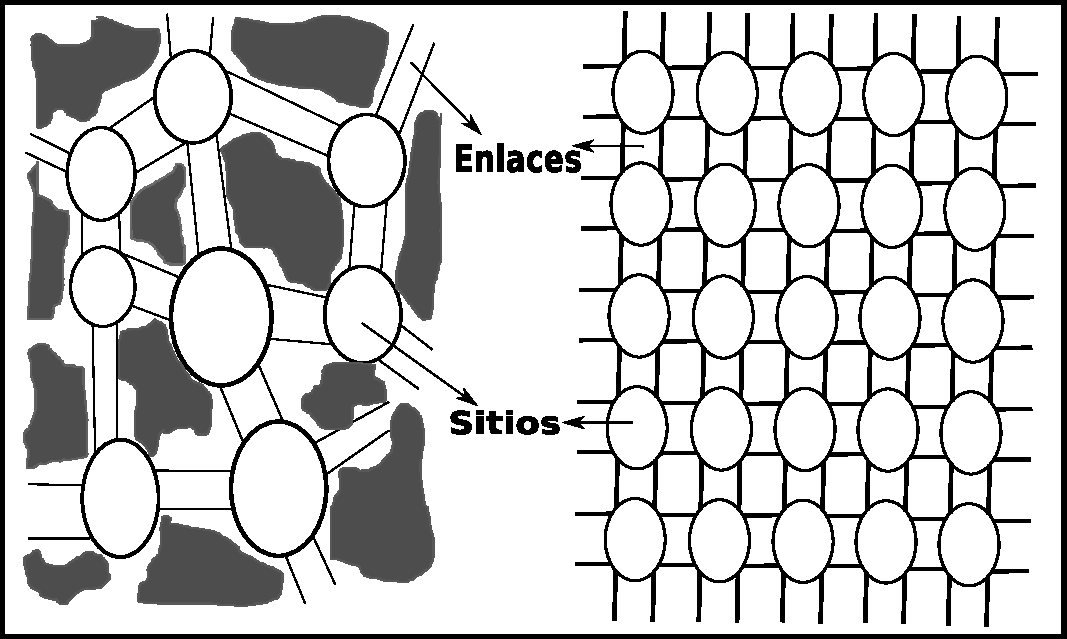
\includegraphics[width=3.5in]{img/dsbm_es.pdf}
\caption{Representación bidimensional de un material poroso mediante el MDSE}
\label{fig:dbsm}
\end{figure}

En este trabajo y como también se utiliza en \cite{ref2}, \cite{ref3} y \cite{ref4}, definimos una red porosa como una matriz cúbica la cual está formada por un conjunto de elementos; cada elemento contiene un sitio conectado a tres enlaces directos, el sitio tambi\'en se conecta a tres enlaces de forma indirecta a través de los sitios vecinos, siguiendo una topología tipo toro tridimensional. Por esto se tiene que cada sitio est\'a conectado directa o indirectamente con seis enlaces, es decir al conectividad de la red es de $C=6$. El tamaño de la red se caracteriza por el parámetro $L$, el cual representa el número de sitos a lo largo de un borde de la matriz cúbica. Con este modelo se tiene que una red de tamaño $L$ contiene $L^3$ sitios y $3L^3$ enlaces (como se muestra en la Figura \ref{fig:lattice3d}).

\begin{figure}[hbtp]
\centering
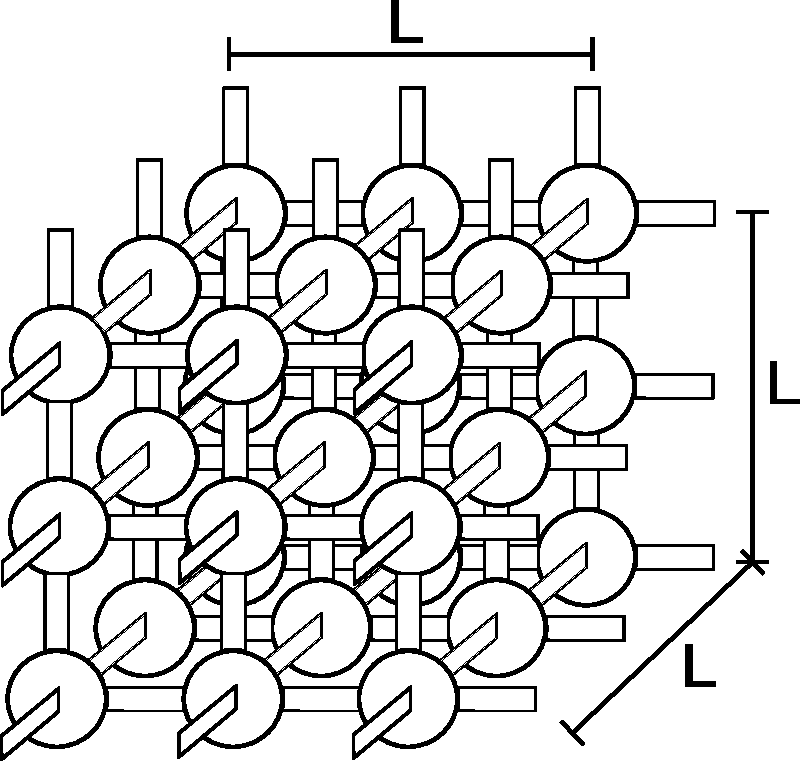
\includegraphics[width=2.8in]{img/red.pdf}
\caption{Red porosa con los sitios representados por esferas y los enlaces representados por cilindros, con $C=6$}
\label{fig:lattice3d}
\end{figure}
 
\section{Principio de Construcción}
\label{sec:mpc}
Un importante aspecto a considerar en la construcción de redes porosas es el Principio de Construcción ($PC$) en el cual se establece que: El tamaño de cada sitio debe ser mayor o al menos igual al tamaño de cualquiera de los enlaces conectados al mismo. Los tamaños de los poros se representan a través de dos distribuciones normales $F_S(R_S)$ para los sitios y $F_B(R_B)$ para los enlaces. $R_S$ es el radio de la esfera que representa a los sitios y $R_B$ es el radio del cilindro que representa a los enlaces. Dada las anteriores distribuciones se sabe que si $FS(RS)$ y $F_B(R_B)$ se traslapan, algunos sitios y enlaces tendrán valores iguales. A esta intersección se le conoce como traslape $\Omega$ (Figura \ref{fig:overlap}). El traslape representa la dificultad de que los sitios y enlaces se conecten de una forma válida, respetando el $PC$. Si $\Omega=0$ esto significa que cualquier enlace es menor que cualquier sitio en términos de tamaño lo que significa que la construcción de una red de poros sería muy sencilla. Por el contrario si $\Omega$ es muy cercano a 1, $F_S(R_S)$ y $F_B(R_B)$ serían muy similares por lo que la asignación de enlaces a los sitios estaría más restringida.\\

\begin{figure}[hbtp]
\centering
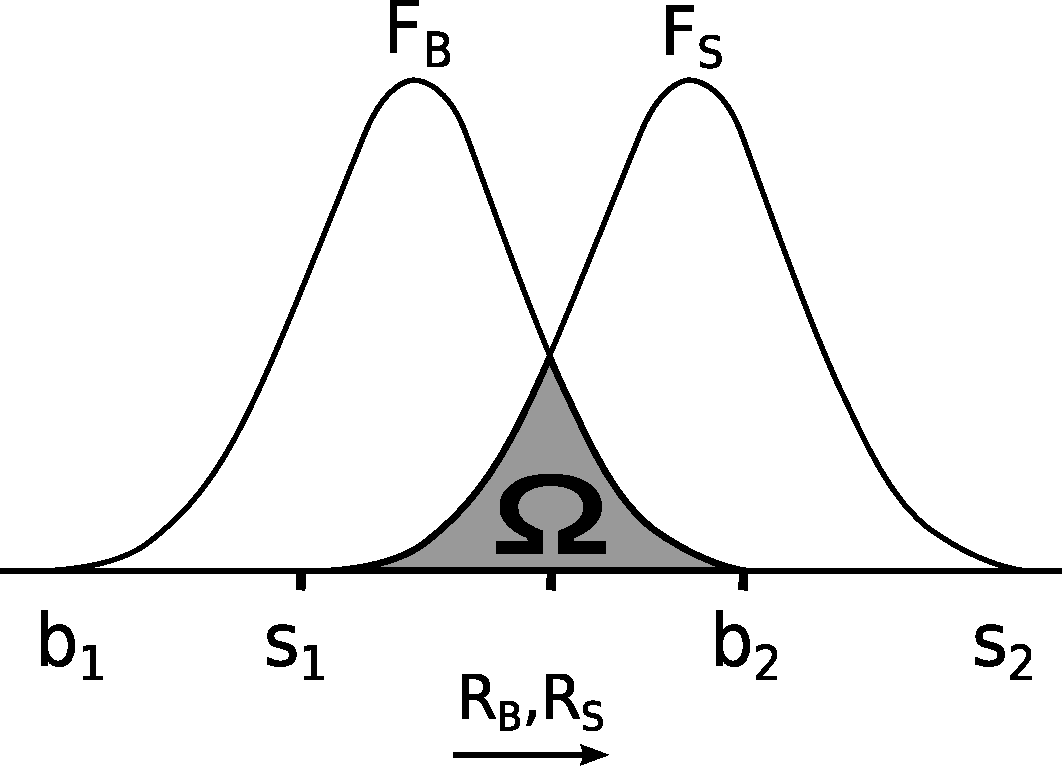
\includegraphics[width=2.5in]{img/traslape.pdf}
\caption{Traslape entre las distribuciones \textit{$F_B$} y $F_S$}
\label{fig:overlap}
\end{figure}

\section{Restricciones Geométricas}
\label{sec:mgr}

En la mayor parte de los trabajos relacionados con la creación de redes porosas solo se basan en el $PC$ para determinar si una red porosa es válida; sin embargo para obtener redes porosas que se asemejen más a la realidad se deben considerar las Restricciones Geométricas ($RG$) entre sitios y enlaces, lo que complementa al $PC$. Al obtener redes porosas más reales las simulaciones tienen mayor exactitud y los experimentos basados en las mismas tienen mayor probabilidad de éxito.\\

Para que una red porosa est\'e sujeta a $RG$ se debe cumplir que para cada enlace conectado aun sitio determinado no debe solaparse con otro enlace conectado al mismo sitio, tal y como se muestra en la Figura \ref{fig:CPyGR}. Las restricciones geométricas se aplican cuando se crea una red porosa consistente, mediante el establecimiento de que para cada par de enlaces vecinos conectados a un sitio, la suma de los cuadrados de sus radios debe ser menor (o a lo más igual) que el cuadrado del sitio. Esto se expresa en la Ecuación \ref{eq:eq01}, donde $i$, $j$ varían desde $1$ hasta $6$.\\

\begin{equation}
R_{B}^2[i]+R_{B}^2[j] \leq R_{S}^2
\label{eq:eq01}
\end{equation}

\begin{figure}[hbtp]
\centering
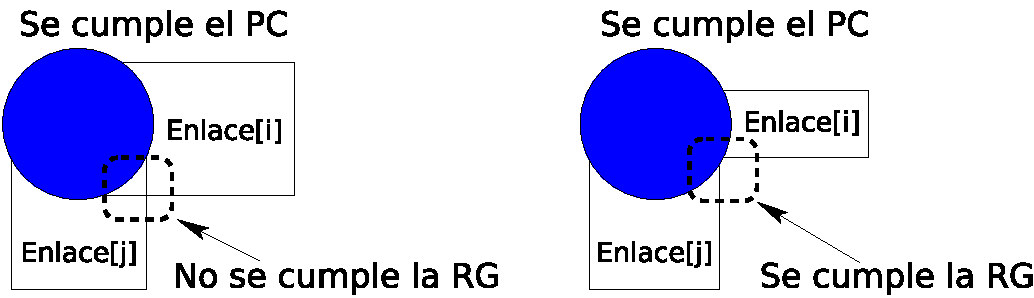
\includegraphics[width=4.0in]{img/CPyGC_es.pdf}
\caption{Representación del $PC$ y $RG$ en un sitio con dos enlaces vecinos}
\label{fig:CPyGR}
\end{figure}

La creación de redes porosas de gran tamaño requiere de grandes recursos de cómputo debido a que un medio poroso esta compuesto por millones, billones, trillones o más poros por unidad de masa, es por eso que se requieren de soluciones eficientes  para poder simular redes porosas de gran tamaño. Debido al volumen de datos que se maneja en las redes porosas las capacidades de cómputo que se necesitan son realmente grandes, lo que se traduce a tiempos de ejecución muy largos. Para dar solución a este problema se pueden aplicar soluciones paralelas para la creación de redes porosas y de esta forma disminuir los tiempos de ejecución y aprovechar las arquitecturas actuales, algunos ejemplos de implementaciones paralelas se pueden ver en \cite{ref4}.\\

\chapter{Objetivos}
\label{champ:objetivos}
\bigskip
\barra
\bigskip


El objetivo principal de  este trabajo es proponer e implementar un sistema eficiente para la simulaci\'on de Redes Porosas sujetas a Restricciones Geométricas.  En el presente trabajo se plantea el desarrollo de un sistema paralelo que saque provecho de las ventajas de las arquitecturas multicore y la programación paralela sobre memoria compartida para acelerar el tiempo de construcci\'on de las redes porosas.

\section{Objetivos Particulares}
\label{sec:objetivosp}
\begin{itemize}
%\item \textbf{Diseñar e implementar algoritmos paralelos basados en dos m?todos secuenciales de creación de redes porosas sujetas a restricciones geométricas: Algoritmo H?brido y M?todo de Monte Carlo}. 
%Este objetivo se realizo implementando dos nuevas versiones para la construcción de redes porosas basándonos en el Modelo Dual de Sitios y Enlaces. La diferencia entre las dos versiones es que en una se utilizo una inicialización aleatoria de sitios y enlaces, y en la otra se intentan conectar los sitios de mayor tamaño con los enlaces más grandes. En ambas versiones se toman en cuenta las $RG$ al conectar sitios y enlaces.

%Ambas versiones se integran de dos grandes pasos que son inicialización y generación de una red porosa válida, en la primera versión la inicialización es completamente aleatoria mientras que en la segunda se hace de tal forma que los enlaces de mayor tamaño se intenten conectar en primera instancia con los enlaces de mayor tamaño, para la generación de una red porosa válida es decir la red cumple completamente son las $RG$ se utiliza el Método de Monte Carlo \cite{ref15}. En ambas versiones se toman en cuenta las $RG$ al conectar sitios y enlaces.

\item {Diseñar e implementar un algoritmo para el particionamiento din\'amico de datos en un sistema multi-core}.
% En base a un análisis de los algoritmos secuenciales y datos de una red porosa, se determino dividir la red porosa en pequeñas subredes siguiendo la metodología divide y vencerás por lo cual el particionamiento de los datos genera suberedes lo más parecidas aun cubo adicionalmente este tipo de particionamiento nos ayudo a disminuir la sincronización entre los hilos.  

\item {Proponer una pol\'itica de distribuci\'on din\'amica de datos para permitir la transferencia de poros entre los procesadores}. 
%Una vez que se tuvo el esquema de particionamiento se paralelizo cada versión secuencial en dicha paralelización. Los algoritmos paralelos fueron diseñados para que cada hilo(tarea computacional) trabajen de forma independiente y sólo se sincronizen en puntos críticos y necesarios.

\item {Obtener una comparaci\'on de los m\'etodos paralelos propuestos identificando sus ventajas y desventajas}. 
%Para validar que un red porosa es válida se verifico que los enlaces conectados a cada sitio cumplieras con las $RG$ recordando que cada sitio tiene tres enlaces propios y tres compartidos siguiendo una topología tipo toro. Para la validación del perforación de los algoritmos secuenciales y paralelos se promedio el tiempo de ejecución de diez pruebas con los mismos datos de entrada para cada algoritmo. 
\end{itemize}






%\chapter{Introducción}
%\label{champ:intro}
%\bigskip
%\barra
%\bigskip
%
%\section{Computo Paralelo y Simulación por Computadora}
%\label{sec:cp}
%
%Por años se han utilizado las computadoras como herramientas para la solución, aproximación o simulación de problemas científicos reales, los cuales tienen una o varias de las siguientes características: son complejos, requieren de un gran número de cálculos o manipulan grandes volúmenes de datos. Lo anterior fue la razón por la cual nació la computación científica la cual es una actividad multidisciplinaria en la cual se hacen uso de métodos y técnicas computacionales para dar soluciones exactas o aproximadas con la premisa de que al utilizar las computadoras el tiempo para obtener resultados es menor. Por lo general la computación científica hace uso  del computo de alto rendimiento(computo paralelo) a través de modelos de programación paralela, los cuales permiten disminuir el tiempo para obtener resultados así como el uso eficiente de los recursos computacionales.\\
%
%La simulación por computadora es una herramienta altamente utilizada debido a que nos permite obtener soluciones aproximadas sobre escenarios de la vida real, varios ramas de la ciencia hacen uso de simulaciones por computadora para lograr mejores resultados en experimentos reales basándose en la información obtenida de simulaciones. Cuando se habla de simulación por computadora esta inherente que se requiere de un modelo el cual nos ayude a abstraer características y limitaciones de un problema real. Adicionalmente de que la simulación por computadora nos permite generar experimentos con mayor exactitud esta también nos puede ayudar a disminuir riesgos y ahorrar recursos.\\
%
%El computo paralelo fue posible gracias a los avances tecnológicos como lo fueron las computadoras multi-procesador o los primeros clusters(Beowulf), en ambas arquitecturas hubo un avance significativo en la primera fue la incorporación de más de un procesador en una misma tarjeta y en la segunda fue el uso de la capacidad de cómputo de computadoras independientes a través de su interconexión(cluster). En la actualidad el computo paralelo va cobrando mayor fuerza y ademas conforme pasa tiempo se esta volviendo más accesible y por lo mismo se esta aplicando en un mayor número de áreas de conocimiento. En particular para aplicar el computo paralelo en un problema se requiere elegir una arquitectura y un técnica de programación. Las arquitecturas más utilizadas para el cómputo paralelo o de alto rendimiento son: multi-procesador, multi-núcleo, gpus, clusters y grids. Por su parte sobre técnicas de programación lo podemos dividir en 3 grandes grupos: la programación con memoria compartida o la programación con memoria distribuida o programación híbrida. 
%
%
%
%Algunos ejemplos donde se ha aplicado el cómputo paralelo para dar una solución en un menor tiempo son: problemas matemáticos , problemas de optimización, así como la simulación de problemas de diversas aréas de conocimiento por mencionar algunos. 
%
%
%En cuanto a la simulación por computadora
%
%%\cite{mchybrid}
%%\cite{mcmulticore}
%%\cite{mcdynamically}
%%
%%\cite{sibalancing}
%%\cite{sicloud}
%%\cite{sikdtree}
%%\cite{silscale}
%%\cite{sinfusion}
%%\cite{siovercomming}
%%\cite{siprocess}
%
%Tanto en \cite{mchybrid} y \cite{mcmulticore} hacen uso de las arquitecturas multi-núcleo sobre memoria compartida para la solución de un problema algebraico y de optimización respectivamente.
%
%
%Una de las ventajas más notables de la programación mediante memoria compartida en arquitecturas multi-núcleo(CPU) es que la comunicación entre los CPUs y la memoria no supone un cuello de botella es por esto que sigue siendo una de las alternativas para paralelizar un algoritmos. Por ejemplo en 
%
%
%En este trabajo se hace uso de una arquitectura multi-núcleo y la técnica de programación utilizada es con memoria compartida.\\
%
%
%Cuando se utilizan arquitecturas multi-núcleo la programación paralela se realiza a través de hilos(tareas computacionales), dos de las tecnologías más utilizadas para el manejo de hilos son: Posix Threads\cite{ref13} y OpenMP\cite{ref6}, ambos siguen el modelo fork-join, sin embargo OpenMP proporciona una interfaz de alto nivel que permite al programador concentrar la mayor parte del tiempo en resolver el problema aplicando algún modelo de programación paralela y no en aspectos técnicos que en ocasiones generan errores que no se relacionan con el problema que se quiere resolver. Ademas OpenMP es un estándar avalado por diversas empresas internacionales y se encuentra soportado por los principales compiladores de C/C++ y Fortran.\\
%
%En particular este proyecto hace énfasis en la simulación de materiales porosos, donde tal y como su nombre lo dice son materiales que tienen poros o huecos, estos poros son de distintos tamaños y se encuentran distribuidos en todo el material con la peculiaridad de que dichos poros se encuentran conectados entre si. Debido a las características que tienen los materiales porosos son altamente utilizados en la industria, al estudiar la estructura y propiedades de estos materiales y adicionalmente con la simulación por computadora se pueden encontrar nuevas aplicaciones y usos industriales.\\
%
%\section{Construcción de Redes Porosas}
%\label{sec:costruction}
%
%\subsection{Modelado de Redes Porosas}
%\label{subsec:model}
%Existen diversos modelos para la simulación de materiales porosos algunos se enfocan en los procesos o fenómenos que suceden dentro de los mismos y otros en la representación del material por si mismo, este último tiene la ventaja de que además de poder conocer las características especificas del material también podemos simular procesos y fenómenos dentro del mismo. Uno de los modelos teóricos para obtener un adecuada descripción de la estructura y propiedades de un medio poroso es el Modelo Dual de Sitios y Enlaces(MDSE)\cite{ref2}, en este modelo existen dos tipos de huecos o poros: sitios y enlaces, donde cada sitio está conectado con un determinado número de enlaces llamado conectividad de la red($C$).\\
%
%La representación Modelo Dual de sitios y Enlaces(MDSE) se puede observar en la Figura \ref{fig:dbsm} en la cual se observa la representación de un medio poroso. Existen varias aplicaciones relacionadas con el MDSE algunas de ellas se reportan en \cite{ref8} y \cite{ref10}. En particular los algoritmos presentados en \cite{ref2}, \cite{ref3} y \cite{ref4} para la creación de redes porosas y en \cite{ref7} para la simulación de la porosimetría del mercurio se basan en el MDSE \cite{ref1}. Cada enlace permite la conexión entre dos sitios, en la Figura \ref{fig:dbsm} se observa una representación en dos dimensiones del MDSE.
%
%\begin{figure}[hbtp]
%\centering
%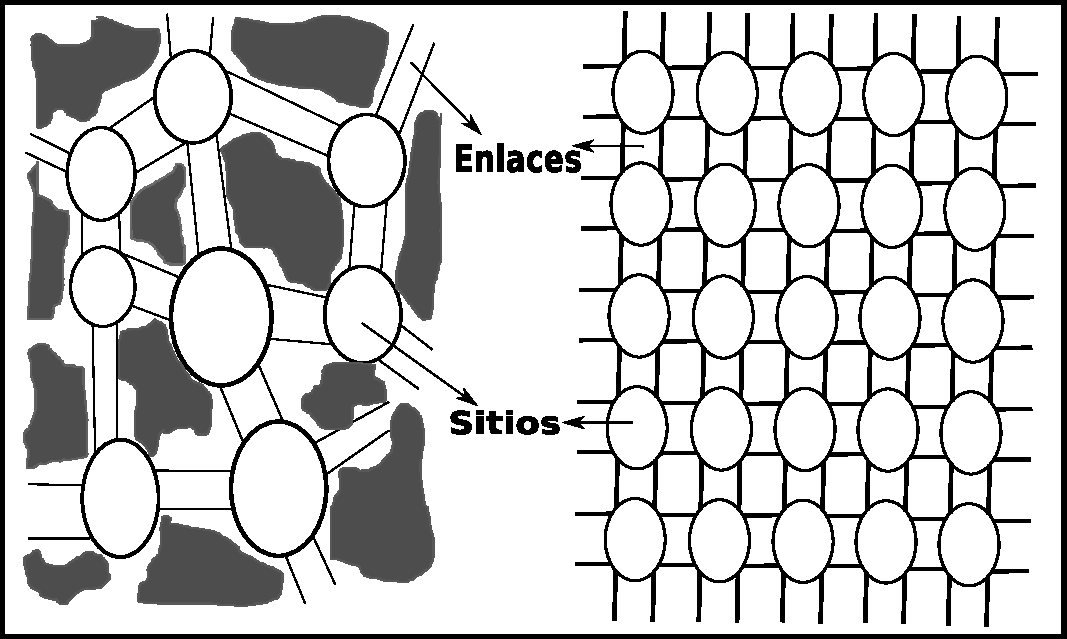
\includegraphics[width=3.5in]{img/dsbm_es.pdf}
%\caption{Representación de un material poroso mediante el MDSE}
%\label{fig:dbsm}
%\end{figure}
%
%En este trabajo y como también se utiliza en \cite{ref2}, \cite{ref3} y \cite{ref4}, definimos una red porosa como una matriz cúbica la cual está formada por la conexión de sitios y enlaces, donde cada sitio se encuentra conectado a tres enlaces directos y a tres enlaces de forma indirecta a través de los sitios vecinos siguiendo una topología tipo toro, por lo que se tiene que cada sitio esta conectado directa o indirectamente con seis enlaces es decir al conectividad de la red es de 6($C=6$). El tamaño de la red se caracteriza por el parámetro $L$, el cual representa el número de sitos a lo largo de un borde de la matriz cúbica. Con este modelo se tiene que una red de tamaño $L$ contiene $L^3$ sitios y $3L^3$ enlaces (Figura \ref{fig:lattice3d}).
%
%\begin{figure}[hbtp]
%\centering
%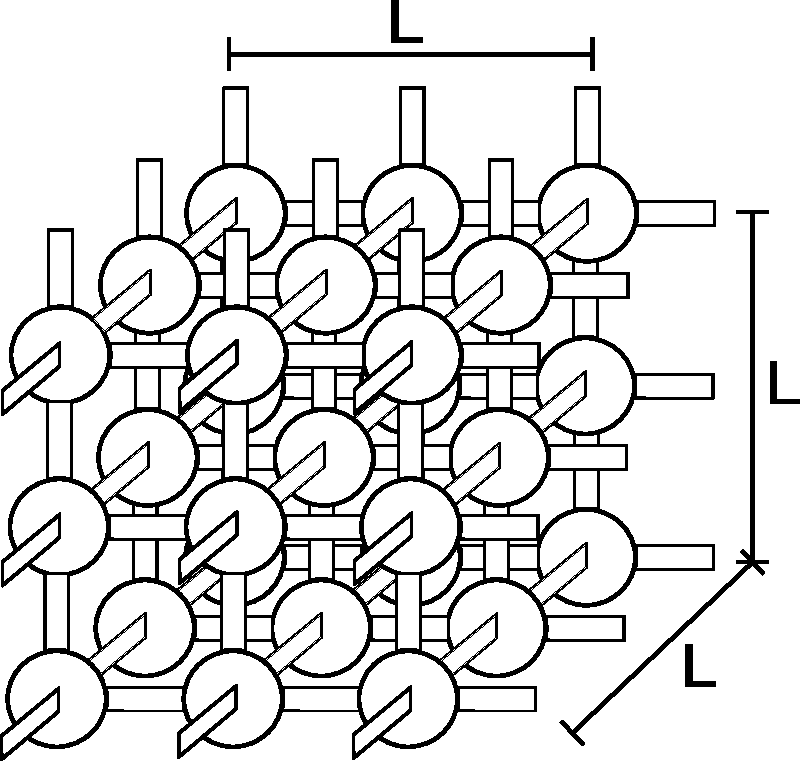
\includegraphics[width=2.8in]{img/red.pdf}
%\caption{Red porosas con los sitios representados por esferas y los enlaces representados por cilindros}
%\label{fig:lattice3d}
%\end{figure}
% 
%\subsection{Principio de Construcción}
%Unos de los método para la construcción de redes porosas es el Principio de Construcción ($PC$) en el cual se establece que: El tamaño de cada sitio debe ser mayor o al menos igual al tamaño de cualquiera de los enlaces conectados al mismo. Los tamaños de los poros se representan a través de dos distribuciones normales $F_S(R_S)$ para los sitios y $F_B(R_B)$ para los enlaces. $R_S$ es el radio de la esfera que representa a los sitios y $R_B$ es el radio del cilindro que representa a los enlaces. Dada las anteriores distribuciones se sabe que si $FS(RS)$ y $F_B(R_B)$ se traslapan, algunos sitios y enlaces tendrán valores iguales. A esta intersección se le conoce como traslape $\Omega$ (Figura \ref{fig:overlap}). El traslape representa la dificultad de que los sitios y enlaces se conecten de una forma válida, respetando el $PC$. Si $\Omega=0$ esto significa que cualquier enlace es menor que cualquier sitio en términos de tamaño lo que significa que la construcción de una red de poros sería muy sencilla. Por el contrario si $\Omega$ es muy cercano a 1, $F_S(R_S)$ y $F_B(R_B)$ serían muy similares por lo que la asignación de enlaces a los sitios estaría más restringida.\\
%
%\begin{figure}[hbtp]
%\centering
%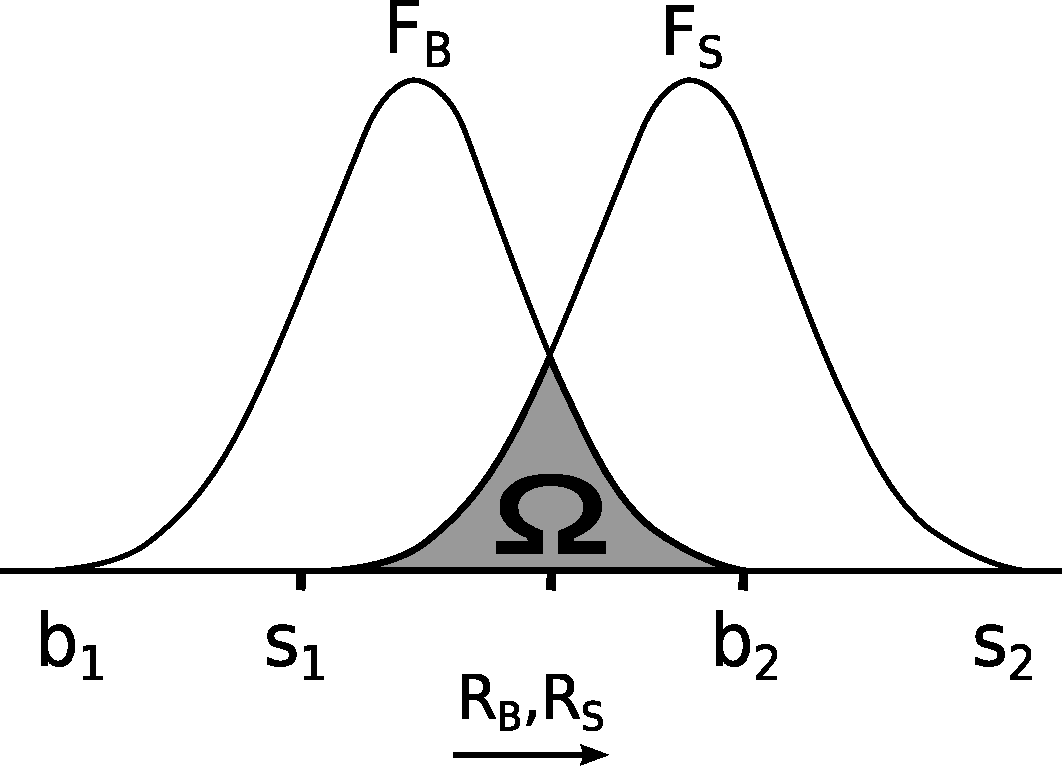
\includegraphics[width=2.5in]{img/traslape.pdf}
%\caption{Traslape entre las distribuciones \textit{$F_B$} y $F_S$}
%\label{fig:overlap}
%\end{figure}
%
%\subsection{Restricciones Geométricas}
%\label{subsec:gr}
%
%En la mayor parte de los trabajos relacionados con la creación de redes porosas solo se basan en el $PC$ para determinar si una red porosa es válida; sin embargo para obtener redes porosas que se asemejen más a la realidad se deben considerar las Restricciones Geométricas ($RG$) entre sitios y enlaces lo que complementa al $PC$, al obtener redes porosas más reales las simulaciones tienen mayor exactitud y por los experimentos basados en las mismas tienen mayor probabilidad de éxito.\\
%
%Para que una red porosa este sujeta a $RG$ se debe cumplir que para cada enlace conectado aun sitio determinado no debe solaparse con otro enlace conectado al mismo sitio, tal y como se muestra en la Figura \ref{fig:CPyGR}. Las restricciones geométricas surgen cuando se crea una red porosa consistente, mediante el establecimiento de que para cada par de enlaces vecinos conectados a un sitio, la suma de los cuadrados de sus radios debe ser menor (o a lo más igual) que el cuadrado del sitio. Esto se expresa en la Ecuación \ref{eq:eq01}, donde $i$, $j$ varían desde $1$ hasta $6$.\\
%
%\begin{equation}
%R_{B}^2[i]+R_{B}^2[j] \leq R_{B}^2
%\label{eq:eq01}
%\end{equation}
%
%\begin{figure}[hbtp]
%\centering
%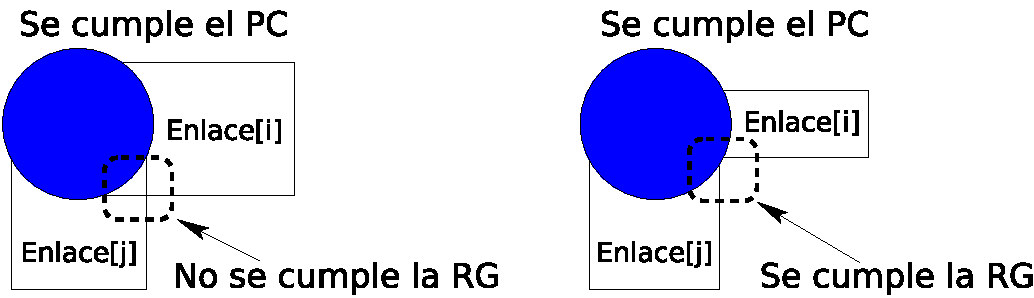
\includegraphics[width=4.0in]{img/CPyGC_es.pdf}
%\caption{Representación del $PC$ y $RG$ en un sitio con dos enlaces vecinos}
%\label{fig:CPyGR}
%\end{figure}
%
%La creación de redes porosas de gran tamaño requiere de grandes recursos de cómputo debido a que un medio poroso esta compuesto por millones, billones, trillones o más poros por unidad de masa, es por eso que se requieren de soluciones eficientes  para poder simular redes porosas de gran tamaño. Debido al volumen de datos que se maneja en las redes porosas las capacidades de cómputo que se necesitan son realmente grandes lo que se traduce a tiempos de ejecución muy largos, para dar solución a este problema se pueden aplicar soluciones paralelas para la creación de redes porosas y de esta forma disminuir los tiempos de ejecución y aprovechar las arquitecturas actuales, algunos ejemplos de implementaciones paralelas se pueden ver en \cite{ref4}.\\
%
%
%\section{Objetivo}
%En el presente trabajo se presenta el diseño e implementación de un sistema paralelo para la construcción de Redes Porosas sujetas a Restricciones Geométricas. El objetivo principal de  este trabajo es el desarrollo de un sistema paralelo que saque provecho de las ventajas de las arquitecturas multicore y la programación paralela sobre memoria compartida.
%
%\subsection{Objetivos Particulares}
%\begin{itemize}
%\item \textbf{Diseñar e implementar dos soluciones secuenciales para la creación de redes porosas sujetas a restricciones geométricas}. Este objetivo se realizo implementando dos nuevas versiones para la construcción de redes porosas basándonos en el Modelo Dual de Sitios y Enlaces. La diferencia entre las dos versiones es que en una se utilizo una inicialización aleatoria de sitios y enlaces, y en la otra se intentan conectar los sitios de mayor tamaño con los enlaces más grandes. En ambas versiones se toman en cuenta las $RG$ al conectar sitios y enlaces.
%
%%Ambas versiones se integran de dos grandes pasos que son inicialización y generación de una red porosa válida, en la primera versión la inicialización es completamente aleatoria mientras que en la segunda se hace de tal forma que los enlaces de mayor tamaño se intenten conectar en primera instancia con los enlaces de mayor tamaño, para la generación de una red porosa válida es decir la red cumple completamente son las $RG$ se utiliza el Método de Monte Carlo \cite{ref15}. En ambas versiones se toman en cuenta las $RG$ al conectar sitios y enlaces.
%
%\item \textbf{Diseñar e implementar un algoritmo para el particionamiento de datos en un sistema multi-core}. En base a un análisis de los algoritmos secuenciales y datos de una red porosa, se determino dividir la red porosa en pequeñas subredes siguiendo la metodología divide y vencerás por lo cual el particionamiento de los datos genera suberedes lo más parecidas aun cubo adicionalmente este tipo de particionamiento nos ayudo a disminuir la sincronización entre los hilos.  
%
%\item \textbf{Diseñar e implementar de un algoritmo paralelo para la construcción de redes porosas sujetas a Restricciones Geométricas}. Una vez que se tuvo el esquema de particionamiento se paralelizo cada versión secuencial en dicha paralelización. Los algoritmos paralelos fueron diseñados para que cada hilo(tarea computacional) trabajen de forma independiente y sólo se sincronizen en puntos críticos y necesarios.
%
%\item \textbf{Validación y Resultados}. Para validar que un red porosa es válida se verifico que los enlaces conectados a cada sitio cumplieras con las $RG$ recordando que cada sitio tiene tres enlaces propios y tres compartidos siguiendo una topología tipo toro. Para la validación del perforación de los algoritmos secuenciales y paralelos se promedio el tiempo de ejecución de diez pruebas con los mismos datos de entrada para cada algoritmo. 
%\end{itemize}
%
%
%\section{Organización de la Idónea Comunicación de Resultados}
%%En el Capítulo \ref{champ:intro} se da una introducción sobre los materiales porosos y algunas de sus aplicaciones, también se habla ligeramente sobre el Principio de Construcción y las Restricciones Geométricas y algunas de las ventajas de estas últimas, adicionalmente se habla u poco sobre el computo paralelo y su aplicación en la simulación por computadora, al final se agrega el objetivo general y los objetivos específicos de este proyecto; 
%
%En el Capítulo \ref{champ:relatedwork} se muestra en forma de resumen el trabajo relacionado en cuanto a algoritmos para la construcción de redes porosas que se basan en MDSE y las ventajas del computo paralelo sobre sistemas de memoria compartida utilizando arquitecturas multi-core. En el Capítulo \ref{champ:BSGR} se presentan dos algoritmos secuenciales para la creación de redes porosas sujetas a las restricciones geométricas. En el Capítulo \ref{champ:PBSGR} se presenta la paralelización de los dos algoritmos secuenciales para la creación de redes porosas sujetas las restricciones geométricas. En el Capítulo \ref{champ:results} se presentan la plataforma de pruebas y los resultados obtenidos así como una análisis de los mismos; por último en el Capítulo \ref{champ:conclusions} se presentan las conclusiones y el trabajo futuro.